\section{Simulation}

\subsection{Signal Generation}
    The audio signal's sampling rate was not enough to simulate the carrier frequency as well. If the original sampling rate was used, we would lose the carrier signal data and end up with a distorted output. Thus, in the simulation, we interpolated the audio file using interp1, and deinterpolated using a time average function at the very end. This wouldn't be necessary in a strictly analog world, but because we're simulating, we need to make several adjustments.

        
    \begin{figure}[H]
        \centering  
        \begin{subfigure}[b]{0.48\textwidth}
            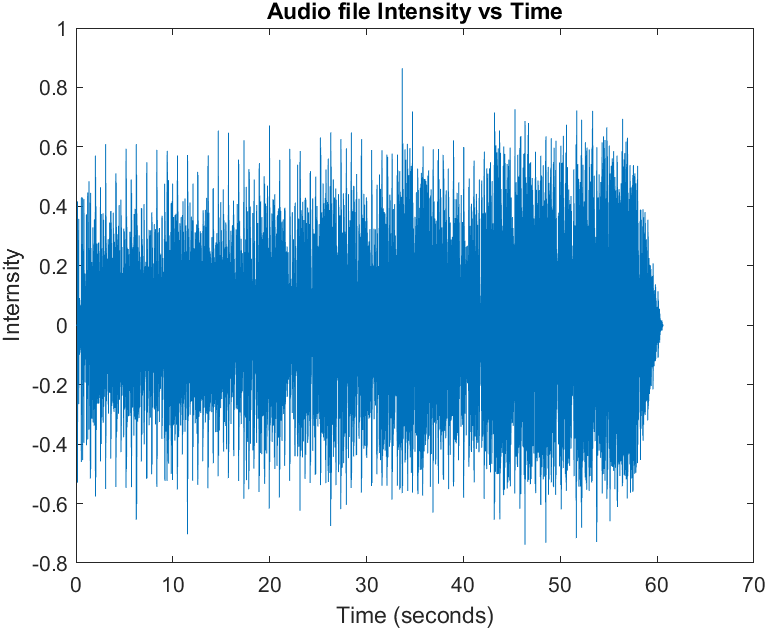
\includegraphics[width=\textwidth]{Images/Audio V Time.png}
            \caption{This audio file has 2,910,576 samples.}
            \label{fig:AudioBeforeInterp}
        \end{subfigure}
        \hfill
        \begin{subfigure}[b]{0.48\textwidth}
            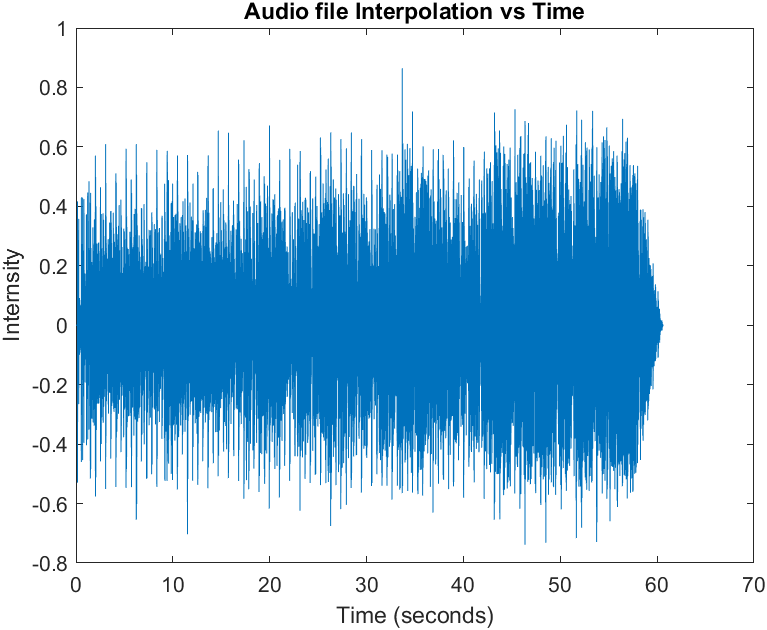
\includegraphics[width=\textwidth]{Images/Audio V Time Interpolated.png}
            \caption{This audio file has 509,350,626 samples.}
            \label{fig:AudioAfterInterp}
        \end{subfigure}
        \caption{Figure \ref{fig:AudioBeforeInterp} should look exactly the same as figure \ref{fig:AudioAfterInterp}, since interpolation will not lose any data.}
    \end{figure}
    
\subsection{Transmitted Wave}
    To simulate the transmission of the wave, we used the standard form of an amplitude modulated wave, as stated in the assignment. However, due to the low signal-to-noise ratio (SNR) in certain parts of the audio, we normalized the audio. This was done by dividing the message by the maximum intensity of the audio.

    \begin{figure}[H]
        \centering  
        \begin{subfigure}[b]{0.48\textwidth}
            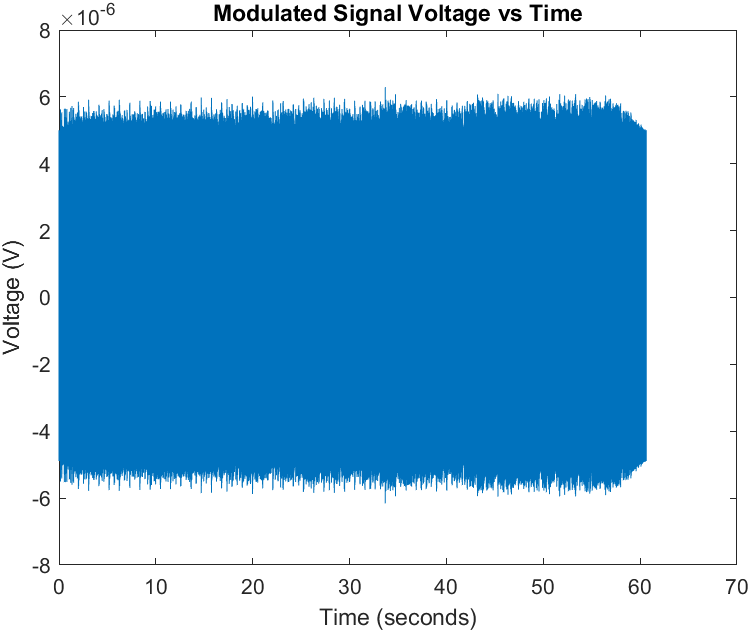
\includegraphics[width=\textwidth]{Images/Modulated Signal Before Normalization.png}
            \caption{Unnormalized Audio}
            \label{fig:AudioBeforeNorm}
        \end{subfigure}
        \hfill
        \begin{subfigure}[b]{0.48\textwidth}
            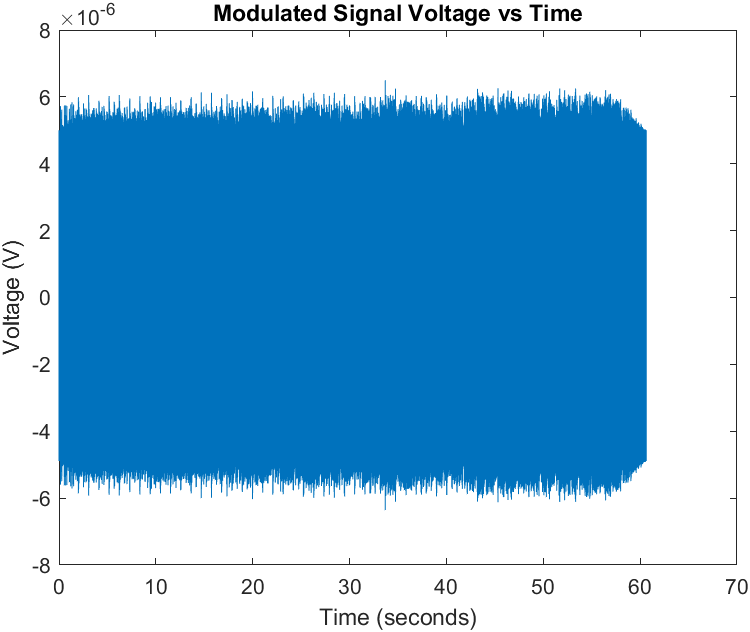
\includegraphics[width=\textwidth]{Images/Modulated Signal After Normalization.png}
            \caption{Normalized Audio}
            \label{fig:AudioAfterNorm}
        \end{subfigure}
        \caption{Figure \ref{fig:AudioBeforeNorm} should look exactly the same as Figure \ref{fig:AudioAfterNorm}, since we are looking on a larger time scale.}
    \end{figure}

\subsection{Amplification}
    In this example, we will assume an absolutely absurd amplification of 1,000,000 once the modulated signal gets to the receiver. We believe that this is also exemplified in the real world, since crystal radios required a special, piezoelectric crystal earpiece which was sensitive to low voltages. However, in the modern world, with high impedance speakers and high voltage sound systems, amplification is necessary.

\subsection{DC Bias}
    The DC Bias was added 
    \begin{figure}[H]
        \centering
        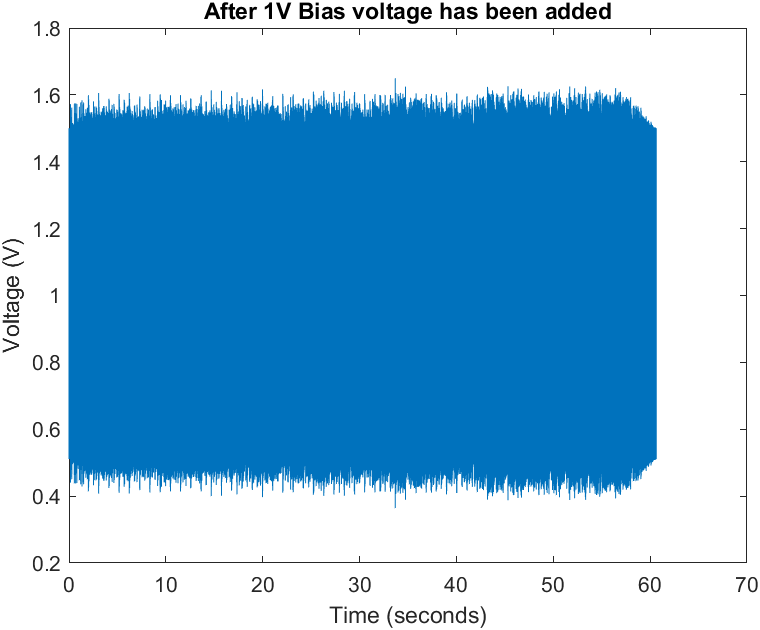
\includegraphics[width=0.5\textwidth]{Images/Bias.png}
        \caption{A 1V Bias voltage has been added}
        \label{fig:Bias}
    \end{figure}
\subsection{Diode}
    The diode was modeled off the practical ideal model of a diode, whose turn on voltage is 0.7. In a perfect world, the diode wouldn't deviate far from its rated forward voltage, so we will assume the perfect world in this report. The MATLAB simulation iterates through each sample. If the input value from the biasing step is lower than 0.7V, it will get recorded as 0. Otherwise, it will be copied over into the new matrix.
    
    Additionally, we decided to model the later high pass filter in this step as well by removing all known DC components. We felt as though this simplified simulation, since the forward voltage drop would be dependant on current through the diode. By not simulating current (Which may change depending on the impedance of the headphones used to listen), we can simulate the ideal scenario. 
    \begin{figure}[H]
        \centering
        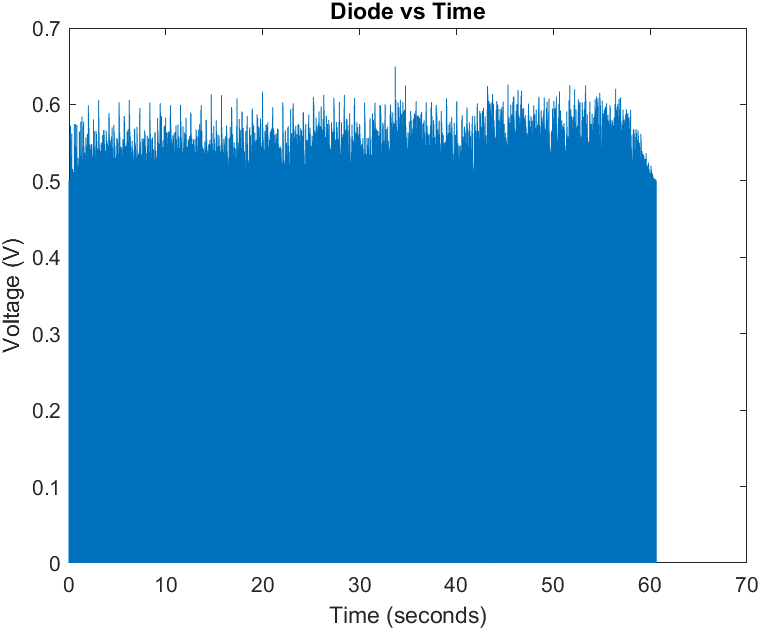
\includegraphics[width=0.6\textwidth]{Images/Diode Signal.png}
        \caption{After the diode. Here, we see all values below 0 are cut off and the signal is now centered at 0.}
        \label{fig:Diode}
    \end{figure}
\subsection{Peak Detector}
    Similar to the diode, the peak detector was modeled by iterating through each sample and comparing its voltage to the previously applied voltage. If the new voltage was higher, the value would simply be copied over to a new matrix. However, if the value was lower, we'd record the last known highest value, as well as the time difference between them. The discharge capacitor equation was then applied to find the new voltage, which was copied to the new matrix. 
    
    \begin{figure}[H]
        \centering
        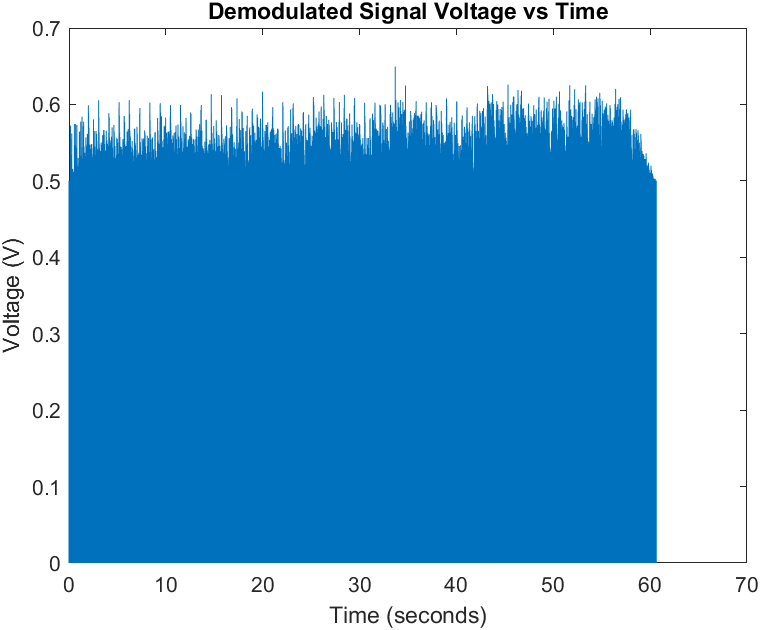
\includegraphics[width=0.6\textwidth]{Images/Demodulated Signal.png}
        \caption{This may look the same as figure \ref{fig:Diode}, but it lacks the 98.6MHz carrier wave. However, this cannot be seen due to the time scale of the audio file used.}
        \label{fig:my_label}
    \end{figure}

\subsection{High-Pass Filter}